\section{Functions}
\subsection{Definition of functions}

A \textbf{function} maps elements of one set $X$ to elements of another set $Y$.
A function from $X$ to $Y$ can be viewed as a subset of $X \times Y : (x, y) \in f$ if $f$ maps $x$ to $y$.
The notation for a function is:
\[
  f: X \rightarrow Y \text{, where $X$ is the \textbf{domain} and $Y$ is the \textbf{co-domain}.}
\]

*if $f$ maps an element of the domain to zero elements \underline{or} more than one element of the target,
then $f$ is \underline{not} \textit{well-defined}

\textbf{Arrow Diagram}:
\begin{align*}
  X & = \{w, x, y, z\} \\
  Y & = \{a, b, c, d\}
\end{align*}

Well-defined functions:
\begin{center}
  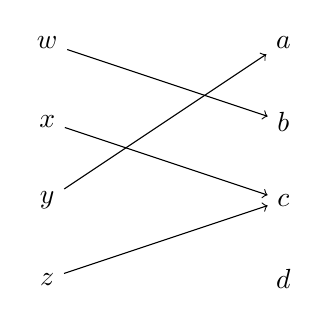
\begin{tikzpicture}
    % domain
    \node (w) at (0, 3) {$w$};
    \node (x) at (0, 2) {$x$};
    \node (y) at (0, 1) {$y$};
    \node (z) at (0, 0) {$z$};
    % co-domain
    \node (a) at (3, 3) {$a$};
    \node (b) at (3, 2) {$b$};
    \node (c) at (3, 1) {$c$};
    \node (d) at (3, 0) {$d$};
    % connections
    \draw[->] (w) -- (b);
    \draw[->] (x) -- (c);
    \draw[->] (y) -- (a);
    \draw[->] (z) -- (c);
  \end{tikzpicture}
  \qquad
  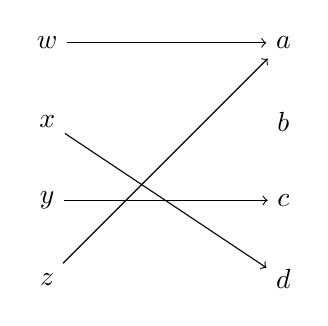
\begin{tikzpicture}
    % domain
    \node (w) at (0, 3) {$w$};
    \node (x) at (0, 2) {$x$};
    \node (y) at (0, 1) {$y$};
    \node (z) at (0, 0) {$z$};
    % co-domain
    \node (a) at (3, 3) {$a$};
    \node (b) at (3, 2) {$b$};
    \node (c) at (3, 1) {$c$};
    \node (d) at (3, 0) {$d$};
    % connections
    \draw[->] (w) -- (a);
    \draw[->] (x) -- (d);
    \draw[->] (y) -- (c);
    \draw[->] (z) -- (a);
  \end{tikzpicture}
\end{center}

\underline{Not} well-defined functions:
\begin{center}
  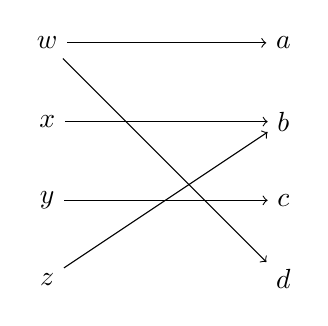
\begin{tikzpicture}
    % domain
    \node (w) at (0, 3) {$w$};
    \node (x) at (0, 2) {$x$};
    \node (y) at (0, 1) {$y$};
    \node (z) at (0, 0) {$z$};
    % co-domain
    \node (a) at (3, 3) {$a$};
    \node (b) at (3, 2) {$b$};
    \node (c) at (3, 1) {$c$};
    \node (d) at (3, 0) {$d$};
    % connections
    \draw[->] (w) -- (a);
    \draw[->] (w) -- (d);
    \draw[->] (x) -- (b);
    \draw[->] (y) -- (c);
    \draw[->] (z) -- (b);
  \end{tikzpicture}
  \qquad
  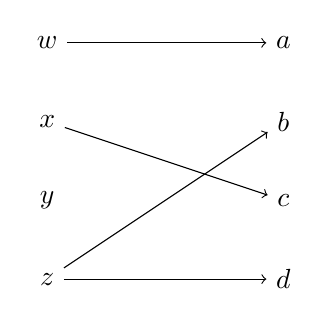
\begin{tikzpicture}
    % domain
    \node (w) at (0, 3) {$w$};
    \node (x) at (0, 2) {$x$};
    \node (y) at (0, 1) {$y$};
    \node (z) at (0, 0) {$z$};
    % co-domain
    \node (a) at (3, 3) {$a$};
    \node (b) at (3, 2) {$b$};
    \node (c) at (3, 1) {$c$};
    \node (d) at (3, 0) {$d$};
    % connections
    \draw[->] (w) -- (a);
    \draw[->] (x) -- (c);
    \draw[->] (z) -- (b);
    \draw[->] (z) -- (d);
  \end{tikzpicture}
\end{center}

For function $f: X \rightarrow Y$, an element $y$ is in the \textbf{range} of $f$
iff there is an $x \in X$ such that $(x, y) \in f$.
\[
  \text{Range of } f = \{y : (x, y) \in f, \text{ for some } x \in X\}
\]
Two functions, $f$ and $g$, are \textbf{equal} if $f$ and $g$ have the same domain and target and
$f(x) = g(x)$ for \underline{every} $x$ in the domain.
\[
  \forall x : f(x) = g(x) \implies f = g
\]

\subsection{Floor and Ceiling functions}

The \textbf{Floor} function, $\left\lfloor x\right\rfloor$
\[
  \text{floor}: \mathbb{R} \rightarrow \mathbb{Z}, \text{ where floor$(x)$ = the largest integer $y$ such that $y \leq x$.}
\]
Notation: $\text{floor}(x) = \left\lfloor x\right\rfloor$
\[\]
\noindent The \textbf{Ceiling} function, $\left\lceil x\right\rceil$
\[
  \text{ceiling}: \mathbb{R} \rightarrow \mathbb{Z}, \text{ where ceiling$(x)$ = the smallest integer $y$ such that $y \geq x$.}
\]
Notation: $\text{ceiling}(x) = \left\lceil x\right\rceil$

\noindent Examples of floor and ceiling:
\begin{align*}
  \left\lceil 4.32\right\rceil  & = 5  & \left\lfloor 4.32\right\rfloor  & = 4  \\
  \left\lceil -4.32\right\rceil & = -4 & \left\lfloor -4.32\right\rfloor & = -5 \\
  \left\lceil 4\right\rceil     & = 4  & \left\lfloor 4\right\rfloor     & = 4  \\
  \left\lceil -4\right\rceil    & = -4 & \left\lfloor -4\right\rfloor    & = -4 \\
\end{align*}

\subsection{Properties of functions}

A function $f: X \rightarrow Y$ is \textbf{one-to-one} or \textbf{injective} if $x_1 \not = x_2$ implies that $f(x_1) \not = f(x_2)$.
$f$ maps different elements in x to different elements in y.

A function $f: X \rightarrow Y$ is \textbf{onto} or \textbf{surjective} if the range of $f$ is equal to the target $Y$.
That is, $\forall y \exists x (y \in Y \land x \in X \land f(x) = y)$

A function $f: X \rightarrow Y$ is \textbf{bijective} if it is both \textbf{injective} and \textbf{surjective}.
A \textbf{bijective} function is called a \textbf{bijection}, or a \textbf{one-to-one correspondence}.

When the domain and target are finite sets, it is possible to infer information about their relative sizes
based on whether a function is one-to-one or onto.
\begin{align*}
  f: D \rightarrow T & \text{ is \textbf{one-to-one}} & \implies &  & \left\lvert D\right\rvert & \leq \left\lvert T\right\rvert \\
  f: D \rightarrow T & \text{ is \textbf{onto}}       & \implies &  & \left\lvert D\right\rvert & \geq \left\lvert T\right\rvert \\
  f: D \rightarrow T & \text{ is \textbf{bijective}}  & \implies &  & \left\lvert D\right\rvert & = \left\lvert T\right\rvert
\end{align*}

\subsection{The inverse of a function}

If a function $f: X \rightarrow Y$ is a \textit{bijection},
then the \textbf{inverse} of f is obtained by exchanging the first and second entries in each pair in $f$.
\begin{align*}
  \text{given } f        & : X \rightarrow Y           \\
  \text{inverse } f^{-1} & : \{(y, x) : (x, y) \in f\}
\end{align*}
Reversing the cartesian pair does not always create a well-defined function.
\textit{Some functions do not have an inverse}.

\textbf{Examples}:
\begin{align*}
  X & = \{1, 2, 3\} \\
  Y & = \{7, 8, 9\}
\end{align*}

\begin{center}
  \begin{tabular}{l}
    $f: X \rightarrow Y$ \\
    $f = \{(1, 7), (2, 9), (3, 9)\}$
  \end{tabular}
  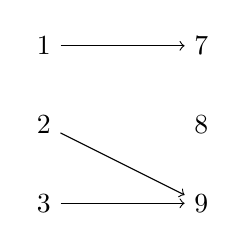
\begin{tikzpicture}
    % domain
    \node (1) at (0, 1) {$1$};
    \node (2) at (0, 0) {$2$};
    \node (3) at (0, -1) {$3$};
    % co-domain
    \node (7) at (2, 1) {$7$};
    \node (8) at (2, 0) {$8$};
    \node (9) at (2, -1) {$9$};
    % connections
    \draw[->] (1) -- (7);
    \draw[->] (2) -- (9);
    \draw[->] (3) -- (9);
  \end{tikzpicture}
  \qquad
  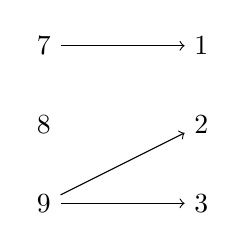
\begin{tikzpicture}
    % domain
    \node (7) at (0, 1) {$7$};
    \node (8) at (0, 0) {$8$};
    \node (9) at (0, -1) {$9$};
    % co-domain
    \node (1) at (2, 1) {$1$};
    \node (2) at (2, 0) {$2$};
    \node (3) at (2, -1) {$3$};
    % connections
    \draw[->] (7) -- (1);
    \draw[->] (9) -- (2);
    \draw[->] (9) -- (3);
  \end{tikzpicture}
\end{center}

\subsection{Composition of functions}
\subsection{Logarithms and exponents}